\begin{frame}
  \maketitle
\end{frame}

\section{本編}
\begin{frame}{背景と目的}
  \begin{itemize}
  \item データセンターにおけるコンピュータネットワークの構造
    \begin{itemize}
    \item 正則(全コンピュータは同一個数のポートを有する)
    \item 短い平均頂点間距離が望ましい\cite{Koibuchi2012,Singla2011}
    \end{itemize}    
  \item 平均頂点間距離の短い正則グラフを求める試み\cite{Fujita2015,Yamamoto2016}
  \end{itemize}
  \begin{columns}[T]
    \begin{column}{.53\textwidth}
      \begin{itemize}
      \item \alert{一般化ムーアグラフ}
        \begin{itemize}
        \item 定義:平均頂点間距離が理論的下界に等しい正則グラフ
          \cite{cerf1973computer, Cerf1974}
        \item 頂点数と次数の組合せによっては存在しない
        \item 探索や存在判定のための効率的方法は知られていない
        \end{itemize}
      \end{itemize}
    \end{column}
    \hspace{\fill}
    \begin{column}{.42\textwidth}
      \begin{figure}
        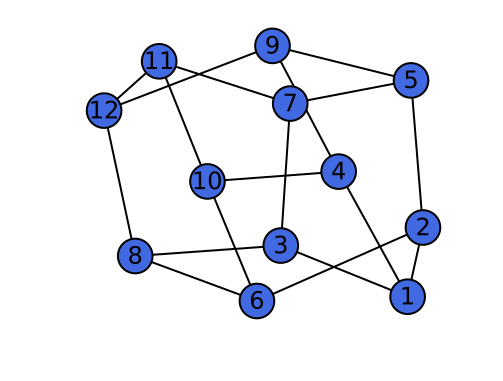
\includegraphics[width=.8\linewidth]{gmg-example-bignode}
        \caption{一般化ムーアグラフの例}
      \end{figure}
    \end{column}
  \end{columns}
  \begin{block}{}
    目的:一般化ムーアグラフの効率的探索法(存在判定法)の提案と評価
  \end{block}
\end{frame}

\begin{frame}{提案する探索法(頂点数12, 次数3の場合)}
\begin{enumerate}
\item 初期グラフの構築(3種類を検討)
\item すべての候補辺(図\ref{fig:feasible-edges-example}の場合は赤い辺)
  を対象に,辺を含めるか否かの判定行う.
  次の条件のうち一つでも満たさなければその先の探索は行わない.
\begin{enumerate}
\item 各頂点の次数が3以下
\item すべての閉路長が5以上
\end{enumerate}
\item すべての辺の判定が終了した後,次の条件を満たすなら探索を終了し,
  一般化ムーアグラフとして出力する.
  \begin{enumerate}
    \item 直径が3以下
  \end{enumerate}
\end{enumerate}
\begin{columns}[b]
\begin{column}{.32\textwidth}
\centering
      \def\svgwidth{\textwidth}
      \input{feasible-edges-example-color.pdf_tex}
      \captionof{figure}{初期グラフ:基本}
      \label{fig:feasible-edges-example}
\end{column}
\begin{column}{.32\textwidth}
\centering
        \def\svgwidth{\textwidth}
        \input{initial-tree-cycle-example.pdf_tex}
        \captionof{figure}{初期グラフ:閉路}
        \label{fig:initial-graph-cycle}
\end{column}
\begin{column}{.32\textwidth}
\centering
        \def\svgwidth{\textwidth}
        \input{initial-spanning-tree-12-example.pdf_tex}
        \captionof{figure}{初期グラフ:全域木}
        \label{fig:initial-graph-stree}
\end{column}
\end{columns}
\end{frame}

\begin{frame}{現在までの成果と今後の計画}
成果
\begin{columns}
\begin{column}{.48\textwidth}
\begin{itemize}
\item 提案法の実装と評価
\begin{itemize}
      \item 初期グラフに全域木を含める場合の探索が最速
      \end{itemize}
\end{itemize}
今後の計画
  \begin{itemize}
  \item より効率的な探索方法の検討
  \item 初期グラフに閉路や全域木の存在を仮定することの妥当性の証明
  \item 同型グラフ判定を用いた列挙
  \item 一般化ムーアグラフの存在判定法の検討
\end{itemize}
\end{column}
\begin{column}{.5\textwidth}
    \includegraphics[width=.95\textwidth]{mid-cmp-algo-time}
      \captionof{figure}{次数3の場合の結果.探索開始から最初の一般化ムーアグラフを発見するまでの時間(10回の試行の平均).}
      \label{fig:result}
    \end{column}
\end{columns}
\end{frame}

\appendix
\begin{frame}<handout:0>{一般化ムーアグラフの条件}
  \begin{thm}
    正則グラフが一般化ムーアグラフであることの必要十分条件は,
    \begin{itemize}
    \item 長さ$2Q$以下の閉路が存在しない
    \item 直径が$Q+1$である($Q+1$層に頂点が存在しない場合は$Q$)
    \end{itemize}
    を同時に満たすことである.
  \end{thm}
  \begin{figure}
    \centering
    \def\svgwith{.4\textwidth}
    \resizebox{.4\textwidth}{!}{
      \input{initial-tree-example.pdf_tex}
    }
    \caption{高さ$Q=2$の木}
  \end{figure}
\end{frame}

\begin{frame}<handout:0>{発見した一般化ムーアグラフの数の比較}
  \begin{columns}
    \begin{minipage}[t]{.5\textwidth}
      \centering
      \includegraphics[height=.65\textwidth]{mid-cmp-algo-full-graph}
      \captionof{figure}{発見したグラフの数 \\ {\scriptsize
          なお,同型なグラフは重複して数えている.
      }}
      \label{fig:full-graph}
    \end{minipage}
    \hspace{1ex}
    \begin{minipage}[t]{.5\textwidth}
      \centering
      \includegraphics[height=.65\textwidth]{mid-cmp-algo-full-time}
      \captionof{figure}{グラフ1個の発見に要した時間 \\ {\scriptsize
          すべてのグラフの発見に要した時間を図\ref{fig:full-graph}の値で
          割った値である.
      }}
      \label{fig:full-time}
    \end{minipage}
  \end{columns}
\end{frame}

\begin{frame}[allowframebreaks]{参考文献}
  \bibliography{../resource/MyCollection}
\end{frame}

